\documentclass[
  a4paper,            % DIN A4
  DIV=10,             % Schriftgröße und Satzspiegel
  oneside,            % einseitiger Druck
  BCOR=5mm,           % Bindungskorrektur
  parskip=half,       % Halber Abstand zwischen Absätzen
  numbers=noenddot,   % Kein Punkt hinter Kapitelnummern
  bibtotoc,           % Literaturverzeichnis im Inhaltsverzeichnis
  listof=totoc        % Abbildungs- und Tabellenverzeichnis im Inhaltsverzeichnis
]{scrartcl}
\usepackage{../style/termpaperstyle}

%\usepackage{layout}       % Layout Debugging
%\usepackage{showframe}    % Layout Debugging
\usepackage{lipsum}       % for example only
\usepackage{blindtext}    % for example only

\begin{document}
% !TEX root = ../termpaper.tex
%
% configurations
%

% text field
%-> replace supervisor names with correct ones
\firstSupervisor{Prof. Dr. Franz Schubert}
\secondSupervisor{}    % only if needed, otherwise left blank

% text field
%-> replace title with your title of the seminar work
\termPaperTitle{Solarbetriebene, mobile Wetterstation}
\termPaperTitleEN{}

% text field
%-> replace the key words with your own key words or remove the words
\keywordsDE{Leben, Universum, Alles}
\keywordsEN{Life, Universe, Everything}

% text field
%-> replace jon with your name
\termPaperAuthor{Isabell Albrecht, Erik Engelhardt, Oliver Kochan, Florian Steffens}

% text field
%-> enter the submission date
\submissionDate{13. Januar 2019}

% switch - uncomment only one
%-> uncomment NDA or public
%\NDA{yes}
\NDA{no}

%-> uncomment cover or cover Corporate Design 2017
%\Cover{CD2017}
%\Cover{CD2017NoLogo}
\Cover{Std2018}

% switch - uncomment only one
%-> uncomment the kind of seminar you are in
\seminarKind{S}     % seminar in bachelor course
%\seminarKind{Pro}   % pro-seminar in bachelor course
%\seminarKind{GSem}  % foundation seminar in master computer science
%\seminarKind{HSem}  % main seminar in master computer science


% switch - uncomment only one
%-> uncomment the study course you are in
%\studycourse{TI}
%\studycourse{AI}
%\studycourse{WI}
%\studycourse{EI}
%\studycourse{BMT}
%\studycourse{MAI}  % master in computer science
%\studycourse{MIK}
%\studycourse{MA}
\studycourse{MES}  

    % load all settings

%\layout{}                 % Layout Debugging

\hyphenation{Ba-che-lor-the-sis Mas-ter-the-sis}

% Cover page here, no page number
\ICoverPage

% Titlepage is page one even if the number is not shown.
\pagenumbering{roman}

% Table of contents here
\newpage
\tableofcontents

% Uncomment if list of source code is needed (rarely).
%\lstlistoflistings  % requires package listings, needs to uncommenting of usepackage

% path to the chapters folder is set to find the images used there
\graphicspath{ {./img/} }

% Chapters
\clearpage
\pagenumbering{arabic}

\begin{abstract}
% !TEX root = ../termpaper.tex
% first example for the abstact
% @author Thomas Lehmann
%
\vspace*{0.4cm}

\noindent Der vorliegende Text ist ein Beispiel für eine Seminararbeit und soll nur die Verwendung des Templates aufzeigen.

\end{abstract}

\ITextBlockKeywords

% !TEX root = ../termpaper.tex
% first example section
% @author Thomas Lehmann
%

\section{Einleitung}

% Add additional chapters here

\section{Ausrichtung des Solarpanels}\label{sec:ausrichtung des Solarpanels}
Um die Leistungsaufnahme des Solarpanels zu optimieren ist es notwendig dieses direkt auf die Sonne auszurichten und diese Ausrichtung auch in geeigneten Zeitabständen zu korrigieren. Im Vergleich mit einem fest ausgerichteten Solarpanel konnten J. Rizek \emph{et al.} mit einem nachgeführten Solarpanel beispielsweise die Leistungsaufnahme um durchschnittlich 30\% erhöhen~\cite{Rizek2008}.

Hierfür kommen grundsätzlich verschiedene Methoden in Frage. In diesen Fall soll die Position der Sonne relativ zur Wetterstation auf Grundlage des Längen- und Breitengrades, der Uhrzeit und des Kalendertages berechnet werden. Diese Information werden über das GPS-Modul bereitgestellt. Anschließend wird das Solarpanel mit Hilfe der Motoren, des Kompass-Moduls und des, am Panel befestigten Neigungssensors, auf die Sonne ausgerichtet.

\subsection{Berechnung der Sonnenposition}\label{sec:berechnung_der_sonnenposition}
Da die Formeln zur Berechnung der Sonnenposition in diesem Projekt lediglich benutzt werden wird an dieser Stelle auf eine Herleitung verzichtet. Die verwendeten Formeln können beispielsweise im \emph{Astronomical Almanac}~\cite{Anon1984} gefunden werden. \emph{M. L. Roderick} beschreibt die nötigen Berechnungen in seinem Report~\cite{Roderick1992} und liefert zudem compilierbaren C-Code. Dieser wird im folgenden zur Berechnung der Sonnenposition verwendet.

Die Position der Sonne im Bezug auf einen Beobachter auf der Erde lässt sich durch die Werte \emph{Zenith} und \emph{Azimut} eindeutig beschreiben. Der Zenith beschreibt den Winkel zwischen einer Linie vom Beobachter zur Sonne und der Vertikalen. Der Azimut den Winkel zwischen der Horizontalen und Norden. Dabei stehen beispielsweise ein Azimut von \SI{90}{\degree} für Osten, \SI{180}{\degree} für Süden und \SI{270}{\degree} für Westen. Eine Veranschaulichung kann in Abbildung~\ref{fig:zen_azi} gefunden werden.

\begin{figure}[H]
  \centering
  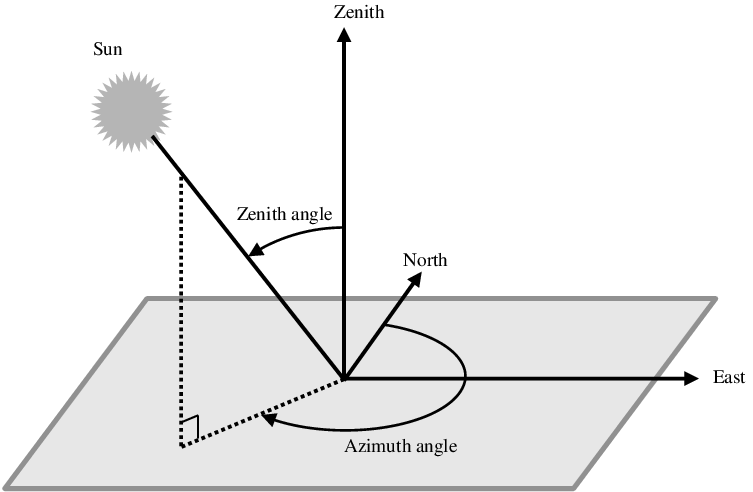
\includegraphics[width=\textwidth]{./img/Representation-of-azimuth-and-zenith-angles.png}
  \caption{Beschreibung der Sonnenposition durch Zenith und Azimut~\cite{Nou2016}}\label{fig:zen_azi}
\end{figure}

Die Genauigkeit der verwendeten Formeln beträgt laut dem \emph{Astronomical Almanac} 


%%% Local Variables:
%%% mode: latex
%%% TeX-master: "../termpaper"
%%% End:

%\bibliographystyle{plain}
\bibliographystyle{dinat}
\bibliography{literature}

%\Istatement

\end{document}

%%% Local Variables:
%%% mode: latex
%%% TeX-master: t
%%% End:
